\chapter{Test und Ergebnisse}
Das Testen ist Zentrales Element im Bereich \ac{rd}. Es ermöglicht die Sicherstellung der Funktionalität der Komponenten und des Systems. In Projekten mit mehreren Gruppenmitgliedern werden die Funktionen durch Teilprojekte gegliedert und Schnittstellen deklariert, wodurch das System modularisiert wird. Somit können für die einzelnen Funktionen und Module sogenannte Unit-Tests\footnote{Komponententest} durchgeführt werden. Nachdem alle Unit-Tests erfolgreich absolviert wurden kann ein Integrationstest\footnote{Systemtest, welcher die einzelnen Module und Funktionen miteinander verbindet} durchgeführt werden. Meist werden an den Systemschnittstellen unter Laborbedingungen definierte Signale angelegt, um die erwartete Reaktion des Systems zu bestätigen. Nach den Labortests erfolgt der Systemtest unter natürlichen Bedingungen in der Umgebung, in dem das System später eingesetzt werden soll, \ac{dh} an den Schnittstellen werden keine definierten Signale mehr angelegt.\\
Auf Grundlage der funktionalen Benutzer- und Systemanforderungen kann mit den Unit- und Integrationstests das System verifiziert werden. Der Unit-Test erlaubt die Überprüfung der funktionalen Software- und Hardwareanforderungen.
\begin{figure}[!h]
	\centering
   	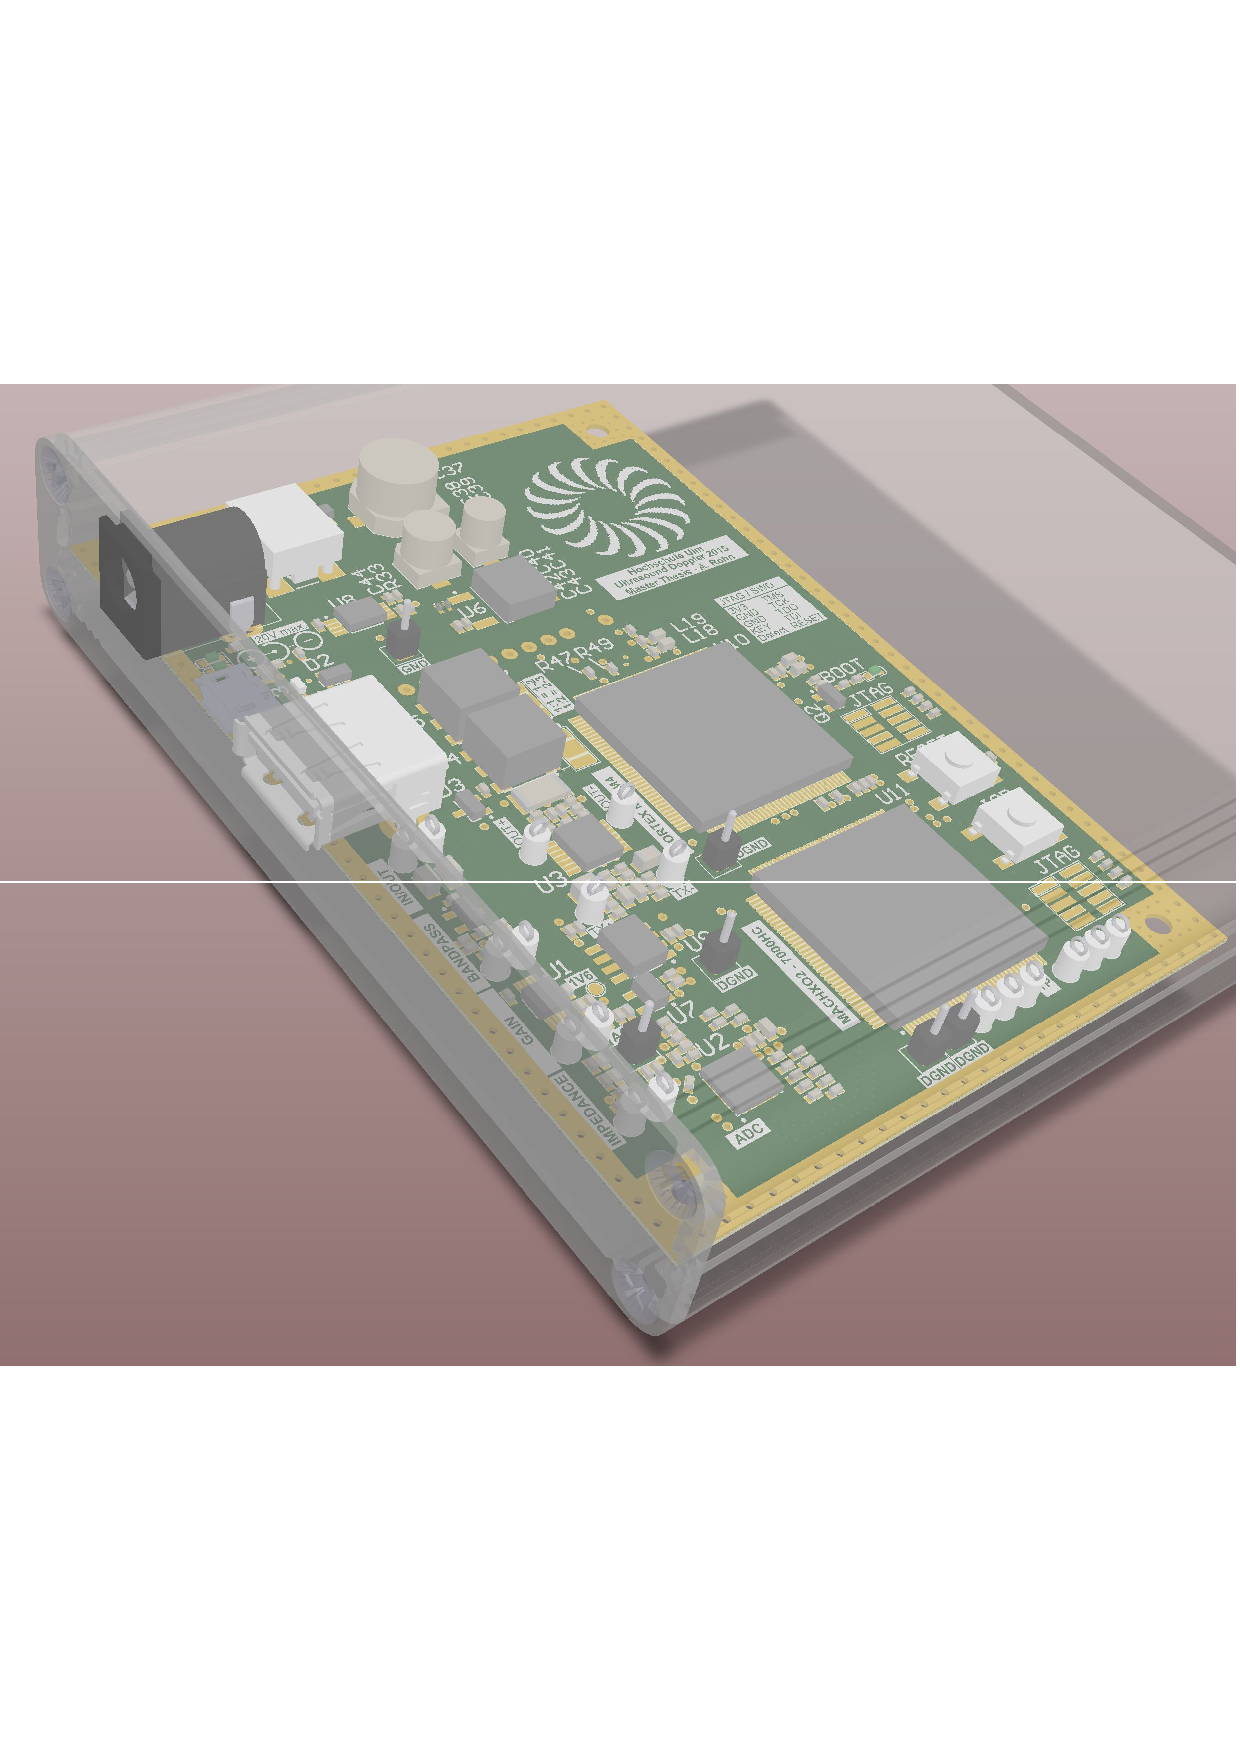
\includegraphics[width=\textwidth, trim= 5mm 65mm 0mm 65mm, clip=true]{images/pcb/Job2.PDF}%docu
    \caption{3D Ansicht der Dopplerinstrumentierung}
    \label{fig:3Dpcb}
\end{figure}
\newpage
\begin{landscape}
\newcommand{\defined}	[1]{& \cellcolor{orange!20}\multirow{#1}{*}{\hfil defined}}
\newcommand{\todo}		[1]{& \cellcolor{red!20}\multirow{#1}{*}{\hfil ToDo}}
\newcommand{\progress}	[1]{& \cellcolor{yellow!20}\multirow{#1}{*}{\hfil in progress}}
\newcommand{\done}		[1]{& \cellcolor{green!20}\multirow{#1}{*}{\hfil done}}
 %param = rows
\newcommand{\userstory}[6]{\cellcolor{orange!20}#1 & \cellcolor{orange!20}#2 & \multirow{#6}{*}{\hfil \cellcolor{orange!20}#3} & \multirow{#6}{*}{\hfil \cellcolor{orange!20}#4 h} & \multirow{#6}{*}{\hfil \cellcolor{orange!20}#5} & \cellcolor{orange!20}}
\newcommand{\task}[6]{ & #1 & \multirow{#6}{*}{\hfil #2} & \multirow{#6}{*}{\hfil #3 h} & \multirow{#6}{*}{\hfil #4} & \multirow{#6}{*}{\hfil #5}}
\newcommand{\test}[6]{\ac{uat} & #1 & \multirow{#6}{*}{\hfil #2} & \multirow{#6}{*}{\hfil #3 h} & \multirow{#6}{*}{\hfil #4} & \multirow{#6}{*}{\hfil #5}}
\
\begin{longtable}{|c|p{115mm}|c|r|c|c|c|}
Nr & Backlog / Task & Priorität & Zeit & Sprint & Bearbeiter & Status \kill
\caption{Produkt Backlog mit Tasks und \acl{uat}s für Hardware Komponenten\label{ProductBacklog_hw}}\\
\hline
\endfirsthead
\caption[]{(Fortsetzung Produkt Backlog mit Tasks und \acl{uat}s für Hardware Komponenten)}\\
\hline
Nr & Backlog / Task & Priorität & Zeit & Sprint & Bearbeiter & Status \\\hline \endhead
Nr & Backlog / Task & Priorität & Zeit & Sprint & Bearbeiter & Status \\\hline
%
%
%
\userstory{HW1}{Als User möchte ich eine Platine für die Ansteuerung meiner Sonde besitzen.}{XL}{352,1}{2}{2} \defined{2}\\
\task{Erstellung eines Schaltplans}{XXL}{170,0}{}{Rehn}{1} \done{1} \\
\task{Erstellung eines \ac{pcb}-Layouts}{XL}{170,0}{}{Rehn}{1} \done{1} \\
\task{\ac{pcb}-Layout an die Herstellmöglichkeiten anpassen}{L}{2,0}{}{Rehn}{1} \done{1} \\
\task{Platine bestellen}{M}{0,5}{}{Rehn, VSK}{1} \done{1} \\
\task{Bauelemente bestellen}{M}{1,5}{}{Rehn, VSK}{1} \done{1} \\
\task{Platine bestücken}{S}{8,0}{}{Rehn, VSK}{1} \progress{1} \\
\test{Die bestückte Platine in der Hand halten und begutachten.}{}{0,1}{}{}{1} \progress{1}\\
\hline
%
%
\userstory{HW2}{Überprüfung der Platine auf richtige Fertigung}{}{0,5}{2}{1} \defined{1}\\
\test{Sichtprüfung der Platine durch Betrachtung der Pinouts und Teardrops unter Hilfenahme eines Mikroskops.}{S}{0,1}{}{Rehn}{3} \done{3} \\
\cline{2-7}
\test{Durchgangsprüfung des Signals DGND an der USB-A Buchse (Designator CON3) auf Layer TOP und BOTTOM zu Signal DGND Einspeisung (Designator J9) auf Layer TOP mit einen Multimeter.}{S}{0,1}{}{Rehn}{3} \done{3} \\
%\cline{2-7}
%\test{Widerstandsmessung der Signale GND, DGND, RXAGND an den Massepins P1-P6 in Bezug zur jeweiligen Referenzeinspeisung mit einen zweipoligen Multimeter.}{S}{0,3}{}{Rehn}{3} \defined{3} \\
\hline
\newpage
%
%
\userstory{HW3}{Überprüfung des Transmitters}{}{x,x}{2}{1} \defined{1}\\
\cline{2-7}
\test{Bei ausgeschalteten Transmitter ein bidirektionales \ac{cpld} Ausgangssignal generieren und an den Messpunkten TX+, TX- und OUT+, OUT- mit Oszilloskop überprüfen, wobei der Trigger auf das Signal TX+ eingestellt wird. Für diesen Test wird der Transmitter durch einen low-Pegel an den \ac{cpld} Pin PT36C und PT36D ausgeschaltet. Ein positives sowie negatives Signal wird an den \ac{cpld} Pins PR2A und PR2B generiert.}{S}{x,x}{}{Rehn}{7} \defined{7} \\
\cline{2-7}
\test{Bei eingeschalteten Transmitter ein bidirektionales \ac{cpld} Ausgangssignal generieren und an den Messpunkten TX+, TX- und OUT+, OUT- mit Oszilloskop überprüfen, wobei der Trigger auf das Signal TX+ eingestellt wird. Für diesen Test wird der Transmitter durch einen high-Pegel an den \ac{cpld} Pin PT36C und PT36D eingeschaltet. Ein positives sowie negatives Signal wird an den \ac{cpld} Pins PR2A und PR2B generiert.}{S}{x,x}{}{Rehn}{7} \defined{7} \\
\cline{2-7}
\test{Bei ausgeschalteten Transmitter jeweils ein positives und ein negatives Signal an den \ac{cpld} Pin PR3A generieren lassen und mit einen Multimeter den additiven Widerstandswert an den Messpunkten OUT+ und OUT- messen. Wenn sich der Widerstandswert ändert, ist die Funktion des PhotoMOS Relays sichergestellt und der Transmitter sollte im Betrieb  mit 2 \ac{mhz} Transducern nicht einbrechen.}{S}{x,x}{}{Rehn}{7} \defined{7} \\
\cline{2-7}
\test{Dauerbelastung des Transmitters durch eine drei minütige Burstphase mit einen Tastverhältnis von 10 bis 50 \% und einer Trägerfrequenz von 2 MHz. Dabei wird besonders auf die Temperaturentwicklung der Leistungswiderstände und auf das Ausgangssignal an den Messpunkten OUT+ und OUT- geachtet.}{S}{x,x}{}{Rehn}{5} \defined{5} \\
\hline
%
%
\userstory{HW4}{Überprüfung des Receivers}{}{0,5}{2}{1} \defined{1}\\
\cline{2-7}
\test{Im spannungsfreien Zustand des Systems wird an den beiden Messpunkten IN/OUT ein Sinussignal von 100 \ac{khz} bis 10 \ac{mhz} in 0,5 \ac{mhz} schritten angelegt. Dabei ist die Amplitude $\geq$ 0,7 Volt einzustellen und es sollte an den Messpunkten BANDPASS mit einen Oszilloskop keine Amplitude gemessen werden.}{S}{x,x}{}{Rehn}{5} \defined{5} \\
\cline{2-7}
\test{Im spannungsfreien Zustand des Systems wird an den beiden Messpunkten IN/OUT ein Sinussignal von 100 \ac{khz} bis 10 \ac{mhz} in 0,5 \ac{mhz} schritten angelegt. Dabei ist die Amplitude $<$ 0,7 Volt einzustellen und es sollte an den Messpunkten BANDPASS mit einen Oszilloskop die Filtercharakteristik bestimmt werden.}{S}{x,x}{}{Rehn}{5} \defined{5} \\
\cline{2-7}
\test{Bei angelegter Spannung an das System wird an den beiden Messpunkten IN/OUT ein Sinussignal von 1 \ac{mhz} bis 10 \ac{mhz} in 0,5 \ac{mhz} schritten angelegt. Zudem ist der \ac{adc} aktiviert und wird mit einen 64 \ac{mhz} Signal betrieben. Dabei ist die Referenzspannung am Messpunkt 1V6 zu überwachen, wodurch die Qualität der analogen Spannungsversorgung ermittelt werden kann.}{S}{0,2}{}{Rehn}{6} \defined{6} \\
\cline{2-7}
\test{Bei angelegter Spannung an das System werden die beiden Messpunkten IN/OUT miteinander Verbunden und somit der differenzielle Eingang des Vorverstärkers kurzgeschlossen. An den Messpunkten GAIN sollten DC Signale anliegen, welche sich um die Referenzspannung 1V6 befinden und konstant bleiben.}{S}{0,3}{}{Rehn}{5} \defined{5} \\
\cline{2-7}
\test{Bei angelegter Spannung an das System wird an den beiden Messpunkten IN/OUT ein Sinussignal von 100 \ac{khz} bis 10 \ac{mhz} in 0,5 \ac{mhz} schritten angelegt. Dabei ist die Amplitude $<$ 0,7 Volt einzustellen und es sollte an den Messpunkten GAIN die gleiche Eingangsfrequenz mit verstärkter Amplitude um den Faktor 20 mit einen Oszilloskop gemessen werden können.}{S}{0,3}{}{Rehn}{7} \defined{7} \\
\cline{2-7}
\test{Bei angelegter Spannung an das System wird an den beiden Messpunkten GAIN miteinander Verbunden und somit der differenzielle Eingang des \ac{adc}s kurzgeschlossen. Mit diesen Test kann die Genauigkeit des \ac{adc}s bestimmt werden, indem an den Serienwiderständen R70 bis R83 des parallen 14-bit Busses \ac{adc}s die Pegeländerungen bei angelegter Messfrequenz von 64 \ac{mhz} bestimmt werden.\footnote{Flatternde Bits}}{S}{0,3}{}{Rehn}{5} \defined{5} \\
\hline
%
%

\end{longtable}
\newpage
%
% SOFTWARE
%
\begin{longtable}{|c|p{115mm}|c|r|c|c|c|}
Nr & Backlog / Task & Priorität & Zeit & Sprint & Bearbeiter & Status \kill
\caption{Produkt Backlog mit Tasks und \acl{uat}s für Software Module\label{ProductBacklog_sw}}\\
\hline
\endfirsthead
\caption[]{(Fortsetzung Produkt Backlog mit Tasks und \acl{uat}s für Software Module)}\\
\hline
Nr & Backlog / Task & Priorität & Zeit & Sprint & Bearbeiter & Status \\\hline \endhead
Nr & Backlog / Task & Priorität & Zeit & Sprint & Bearbeiter & Status \\\hline
%
%
%
\userstory{COM1}{Als User möchte ich mit meiner Platine über die \ac{usb} Schnittstelle kommunizieren.}{XL}{352,1}{2}{2} \defined{2}\\
\task{USB descriptor definieren}{XXL}{0,5}{}{Rehn}{1} \done{1} \\
\task{USB descriptor implementieren}{XXL}{7,5}{}{Rehn}{1} \done{1} \\
\test{Den \ac{usb}-Code auf den Cortex der bestückten Platine flashen und die Platine mit einen USB Kabel an einen \ac{pc} anschließen. Eine automatische Treiberinstallation\footnote{ab Microsoft Windows XP SP2 mit Administratorrechten} sollte automatisch angestoßen und der usb-descriptor mit UsbTreeView vollständig visualisiert werden.}{}{0,2}{}{}{4} \todo{4}\\
\cline{2-7}
%\test{Die \ac{led} an Pin P1_1 des ARM Cortex-M4 über einen Control-Transfer der \ac{usb}-Schnittstelle an- sowie ausschalten.}{}{0,1}{}{}{4} \todo{4}\\
\cline{2-7}
\test{einen 1024 großes 32bit Array im ARM Cortex-M4 anlegen und mit Counterwerten von 0 bis 1023 füllen. Anschließend einen Datenupload zum \ac{pc} über den Control-Transfer initialisieren und über einen Bulk-Transfer (Bulk-In) transferieren. Da die maximale Paketgröße bei \ac{usb} High-Speed 512 byte Pakete beträgt, müssen 8 Transfers übertragen werden. Mit diesen Test kann eine Reihe von Datenpaketen übertragen und somit ein Teil eines Streams simuliert werden, was für den späteren Anwendungsfall benötigt wird.}{}{x,x}{}{}{8} \todo{8}\\
\hline
%
%
\userstory{COM2}{Der ARM Cortex-M4 soll über die \ac{spi} Schnittstelle das \ac{cpld} parametrisieren und diese Parameter auslesen können.}{XL}{352,1}{2}{2} \defined{2}\\
\task{Adressen inklusive Befehle für \ac{cpld} deklarieren.}{XXL}{0,5}{}{Rehn}{1} \done{1} \\
\cline{2-7}
\test{Eine Erfolgreiche Implementierung des ARM Cortex-M4 }{}{0,2}{}{}{4} \todo{4}\\
\test{}{}{0,2}{}{}{4} \todo{4}\\
\test{}{}{0,2}{}{}{4} \todo{4}\\
\cline{2-7}

\end{longtable}
\end{landscape}

\section{Komponententest (Unit-Test)}


\section{Systemtest (Integration-Test)}\label{sec:inttest}
Nachdem die grundlegenden Funktionalitäten verifiziert wurden, konnte das System in Betrieb genommen werden.